\documentclass[preview,border=4mm,convert={density=600,outext=.png}]{standalone}
\usepackage{tikz}
\usetikzlibrary{shapes,snakes}

% Vato
\newcommand{\nodec}[3]{\node[circle,draw,minimum size=20, fill=#3] (#1#2) at (1.5*#1,1.5*#2) {};}

% Dead node -- crossed out in red
\newcommand{\dnode}[3]{
  \nodec{#1}{#2}{#3}
  \node[cross out, draw, thick, color=red] at (1.5*#1,1.5*#2) {};
}

\newcommand{\trace}[2]{\draw[->, dotted, line width=0.1cm, red] (#1)--(#2);}

% laka(length, height, size)
\newcommand{\laka}[3]{
  \foreach \x in {1, ..., #1}
  \foreach \y in {1, ..., #2}
  \node[circle, draw] (\x\y) at (#3*\x, #3*\y) {};
}

\newcommand{\fanorontelo}{  
  \laka{3}{3}{1.5};
  
  \foreach \x [evaluate=\x as \sx using int(\x+1)] in {1, 2}
  \foreach \y  in {1, ..., 3}
  \draw (\x\y)--(\sx\y);

  \foreach \y [evaluate=\y as \sy using int(\y+1)] in {1, 2}
  \foreach \x in {1, ..., 3}
  \draw (\x\y)--(\x\sy);

  \draw (11)--(22) (22)--(33);
  \draw (13)--(22) (22)--(31);

}

\newcommand{\fanorondimy}{
  \laka{5}{5}{1.5};
  
  \foreach \x [evaluate=\x as \sx using int(\x+1)] in {1, ..., 4}
  \foreach \y  in {1, ..., 5}
  \draw (\x\y)--(\sx\y);

  \foreach \y [evaluate=\y as \sy using int(\y+1)] in {1, ..., 4}
  \foreach \x in {1, ..., 5}
  \draw (\x\y)--(\x\sy);

  \foreach \x [evaluate=\x as \sx using int(\x+1),
  evaluate=\sx as \ssx using int(\sx+1)] in {1, 3}{
    \foreach \y [evaluate=\y as \sy using int(\y+1),
    evaluate=\sy as \ssy using int(\sy+1)] in {1, 3, ..., 4}{
      \draw (\x\y)--(\sx\sy) (\sx\sy)--(\ssx\ssy);
    }
  }
  
  \foreach \x [evaluate=\x as \px using int(\x-1),
  evaluate=\px as \ppx using int(\px-1)] in {3, 5}{
    \foreach \y [evaluate=\y as \sy using int(\y+1),
    evaluate=\sy as \ssy using int(\sy+1)] in {1, 3}{
      \draw (\x\y)--(\px\sy) (\px\sy)--(\ppx\ssy);
    }
  }
}

\newcommand{\fanorontsivy}{
  \laka{9}{5}{1.5};
  
  \foreach \x [evaluate=\x as \sx using int(\x+1)] in {1, ..., 8}
  \foreach \y  in {1, ..., 5}
  \draw (\x\y)--(\sx\y);

  \foreach \y [evaluate=\y as \sy using int(\y+1)] in {1, ..., 4}
  \foreach \x in {1, ..., 9}
  \draw (\x\y)--(\x\sy);

  \foreach \x [evaluate=\x as \sx using int(\x+1),
  evaluate=\sx as \ssx using int(\sx+1)] in {1, 3, ..., 8}{
    \foreach \y [evaluate=\y as \sy using int(\y+1),
    evaluate=\sy as \ssy using int(\sy+1)] in {1, 3, ..., 4}{
      \draw (\x\y)--(\sx\sy) (\sx\sy)--(\ssx\ssy);
    }
  }
  
  \foreach \x [evaluate=\x as \px using int(\x-1),
  evaluate=\px as \ppx using int(\px-1)] in {3, 5, ..., 9}{
    \foreach \y [evaluate=\y as \sy using int(\y+1),
    evaluate=\sy as \ssy using int(\sy+1)] in {1, 3}{
      \draw (\x\y)--(\px\sy) (\px\sy)--(\ppx\ssy);
    }
  }  
}


\begin{document}

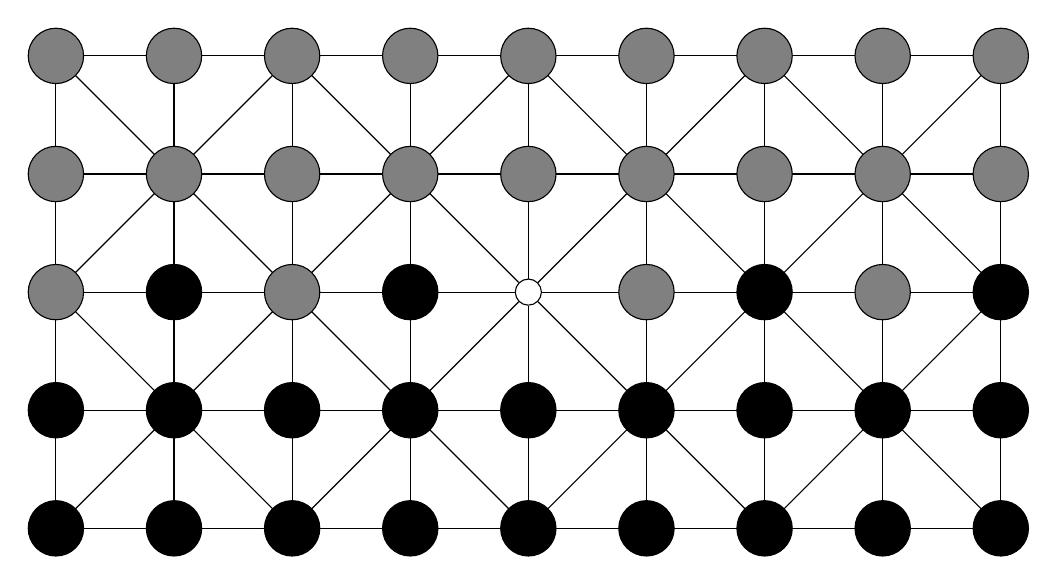
\begin{tikzpicture}

  % % FANORONTELO
  % % ===========
  
  % \fanorontelo{};

  % \nodec{1}{2}{gray};
  % \nodec{1}{3}{gray};
  % \nodec{2}{3}{gray};
  % \nodec{3}{3}{gray};
  % \nodec{1}{1}{black};
  % \nodec{2}{1}{black};
  % \nodec{3}{1}{black};
  % \nodec{3}{2}{black};

  % ----------------------------------------------------------------------------

  % FANORONDIMY
  % ===========
  % \fanorondimy{};
    
  % % Player 1
  % % --------
  
  % \foreach \x in {1, ..., 5}
  % \foreach \y in {4, 5}
  % \nodec{\x}{\y}{gray};

  % \foreach \x in {1, 4}
  % \nodec{\x}{3}{gray};

  % % Player 2
  % % -----------
  
  % \foreach \x in {1, ..., 5}
  % \foreach \y in {1, 2}
  % \nodec{\x}{\y}{black};
  
  % \foreach \x in {2, 5}
  % \nodec{\x}{3}{black};

  % ----------------------------------------------------------------------------

  % % FANORONTSIVY
  % % ============
  
  \fanorontsivy{}
    
  % Player 1
  % --------
  
  \foreach \x in {1, ..., 9}
  \foreach \y in {4, 5}
  \nodec{\x}{\y}{gray};
  
  \foreach \x in {1, 3, 6, 8}
  \nodec{\x}{3}{gray};

  % Player 2
  % -----------
  
  \foreach \x in {1, ..., 9}
  \foreach \y in {1, 2}
  \nodec{\x}{\y}{black};
  
  \foreach \x in {2, 4, 7, 9}
  \nodec{\x}{3}{black};
  
  % Fitaritana
  % ==========

  % Vaky Loha
  % *********
  % \trace{52}{53};
  % \dnode{5}{4}{gray};
  % \dnode{5}{5}{gray};
  
  % Havanana
  % ********  
  % \trace{42}{53};
  % \dnode{6}{4}{gray};
  % \dnode{7}{5}{gray};

  % Havia
  % *****  
  % \trace{62}{53};
  % \dnode{4}{4}{gray};
  % \dnode{3}{5}{gray};

  % Kobaka lava
  % ***********
  % \trace{63}{53};
  % \dnode{7}{3}{black};

  
  % Kobaka fohy
  % ***********
  % \trace{63}{53};
  % \dnode{4}{3}{black};


  % \trace{52}{53}
  % \trace{53}{64}
  % \trace{64}{63}    
 
\end{tikzpicture}
\end{document}

%%% Local Variables: 
%%% mode: latex   
%%% TeX-master: t   
%%% End: